
\documentclass{article}
\usepackage[utf8]{inputenc}
\usepackage{tikz}

\begin{document}

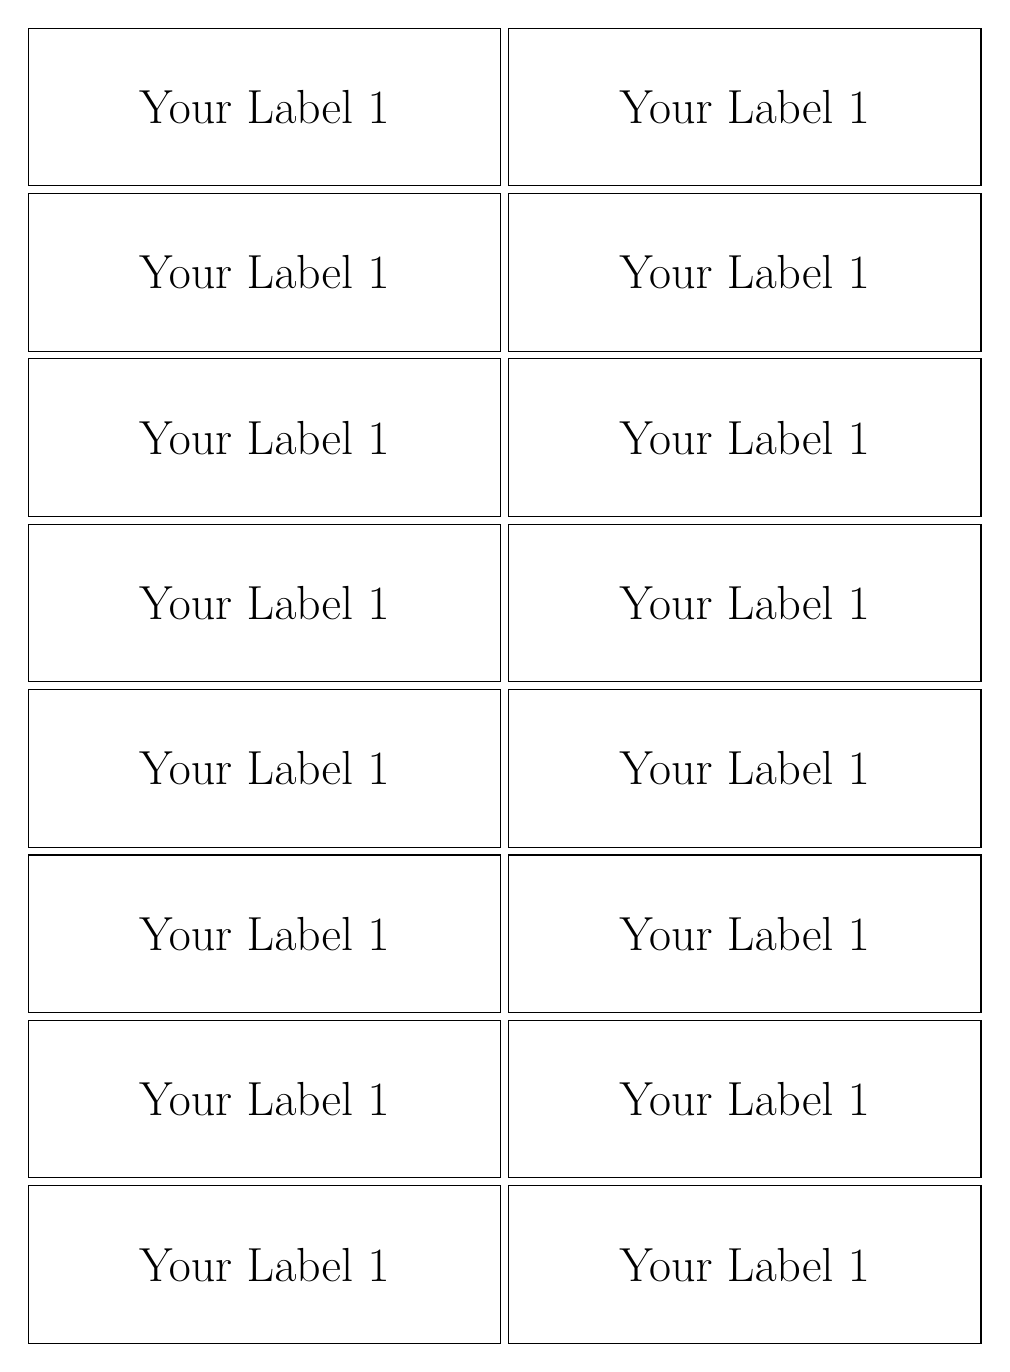
\begin{tikzpicture}[
block/.style={
draw,
fill=white,
rectangle, 
minimum width=6cm,
minimum height=2cm,
font=\LARGE}
]

\draw (0,0)node[block]{Your Label 1};
\draw (6.1,0)node[block]{Your Label 1};
\draw (0,-2.1)node[block]{Your Label 1};
\draw (6.1,-2.1)node[block]{Your Label 1};
\draw (0,-4.2)node[block]{Your Label 1};
\draw (6.1,-4.2)node[block]{Your Label 1};
\draw (0,-6.3)node[block]{Your Label 1};
\draw (6.1,-6.3)node[block]{Your Label 1};
\draw (0,-8.4)node[block]{Your Label 1};
\draw (6.1,-8.4)node[block]{Your Label 1};
\draw (0,-10.5)node[block]{Your Label 1};
\draw (6.1,-10.5)node[block]{Your Label 1};
\draw (0,-12.6)node[block]{Your Label 1};
\draw (6.1,-12.6)node[block]{Your Label 1};
\draw (0,-14.7)node[block]{Your Label 1};
\draw (6.1,-14.7)node[block]{Your Label 1};


\pagenumbering{gobble}
\end{tikzpicture}
\end{document}

